\chapter{Scene Graph Architecture and Hierarchy}
\label{chap:scene_graph}

\section{Scene Graph Architectural Overview}
A flat collection of isolated 3D meshes cannot model complex architectural compositions, moving limbs, or physical assemblies where components are anchored to moving parents. To solve this, \textit{Matsuri Nights} implements an object-oriented hierarchical \textbf{Scene Graph} rooted at \texttt{SceneNode} (\texttt{src/SceneNode.h}).

\begin{figure}[H]
\centering
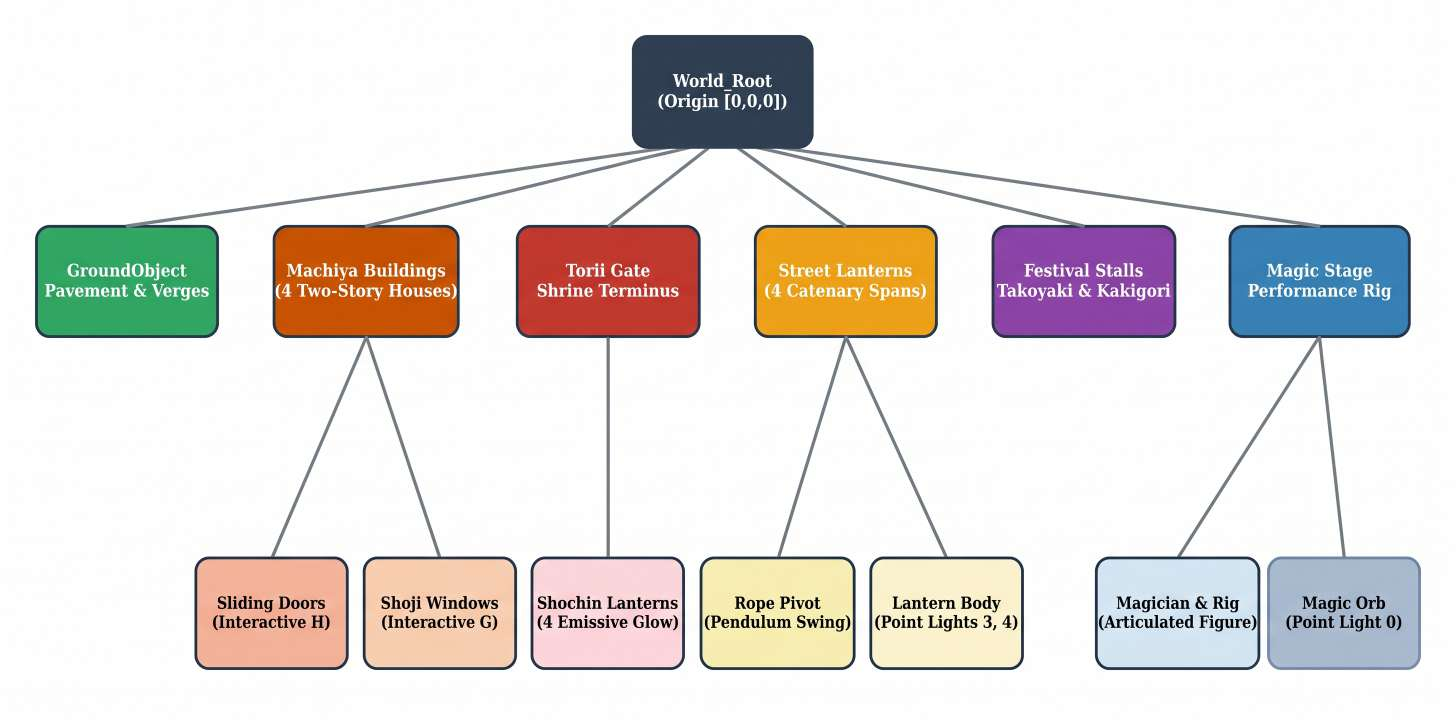
\includegraphics[width=0.95\textwidth]{figures/fig_scene_graph_tree.pdf}
\caption{Hierarchical Scene Graph Tree illustrating the inheritance of spatial reference frames from \texttt{World\_Root} to sub-assemblies.}
\label{fig:scene_graph_tree}
\end{figure}

\section{The SceneNode Class Implementation}
Each node in the scene graph encapsulates spatial, material, and topological state:
\begin{lstlisting}[language=C++, basicstyle=\ttfamily\scriptsize]
class SceneNode : public std::enable_shared_from_this<SceneNode> {
public:
    std::string name;
    Transform transform;              // Local affine transform
    glm::mat4 worldMatrix{ 1.0f };    // Cascaded world transform
    glm::mat3 normalMatrix{ 1.0f };   // Inverse transpose for normals

    SceneNode* parent = nullptr;      // Non-owning back-pointer to parent
    std::vector<std::shared_ptr<SceneNode>> children;

    const Mesh* mesh = nullptr;       // Geometric primitive pointer
    glm::vec4 color{ 1.0f };          // Base diffuse tint
    bool isWindow = false;            // Shoji paper transmission flag
    bool isSky = false;               // Celestial background flag
    bool isEmissive = false;          // Glowing lantern/firework flag
    glm::vec3 emissiveColor{ 0.0f };

    float shininess = 32.0f;          // Blinn-Phong specular power
    float specularStrength = 0.5f;

    const Texture* texture = nullptr; // Diffuse map pointer
    float textureTiling = 1.0f;

    bool isStatic = false;            // Caching optimization flag
    bool castShadow = true;           // Shadow depth pass participation flag
};
\end{lstlisting}

\subsection{Matrix Propagation and Dirty-Flag Optimization}
Computing full matrix cascades for hundreds of nodes every frame incurs severe CPU cache overhead. \texttt{SceneNode} implements an aggressive dirty-flag propagation system (\texttt{updateWorldMatrix}):
\begin{enumerate}
    \item \textbf{Local Transform Inspection:} \texttt{transform.checkDirty()} returns true if position, rotation, or scale changed since the previous evaluation.
    \item \textbf{Parent Change Detection:} The node verifies whether the incoming \texttt{parentMatrix} differs from \texttt{lastParentMatrix}.
    \item \textbf{Early Exit for Static Subtrees:} When \texttt{isStatic} is set to true and neither the node nor its ancestors mutated, matrix re-evaluation and child traversal are entirely skipped.
\end{enumerate}

\subsection{RenderContext and State Cache Minimization}
Calling \texttt{glGetUniformLocation} during the render loop incurs expensive OpenGL driver hash table lookups. To prevent this, \texttt{SceneNode.h} introduces \texttt{RenderContext}:
\begin{itemize}
    \item Uniform locations are queried and stored once during initialization (\texttt{ctx.init(shader)}).
    \item Uniform values (\texttt{lastShininess}, \texttt{lastSpecularStrength}, \texttt{lastTexture}) are cached within the context. Redundant uniform setter calls are bypassed unless the material properties actually change between nodes.
\end{itemize}

\section{Catalog of the 17 Scene Entities}
The complete virtual festival environment is constructed from 17 architectural and animated entities initialized in \texttt{Scene::buildScene()} (\texttt{src/Scene.h}):
\begin{enumerate}
    \item \textbf{Ground (\texttt{GroundObject}):} A 9m wide, 80m long stone cobblestone street flanked by grass verges and granite curbstones.
    \item \textbf{Machiya L1 \& L2 (\texttt{MachiyaBuilding}):} Two traditional 2-story townhouses on the left side of the street featuring sliding Shoji entrance doors, sliding windows, interior Tatami rooms, and curved tile eaves.
    \item \textbf{Machiya R1 \& R2 (\texttt{MachiyaBuilding}):} Symmetrical 2-story townhouses lining the right side of the street.
    \item \textbf{Torii Gate (\texttt{ToriiGate}):} Grand vermilion shrine gate at street terminus ($z = -32.0\,\text{m}$) with curved Kasagi beam, sacred Shimenawa catenary rope, Shide paper streamers, hanging Chochin lanterns, bracket lanterns, and stone Toro lanterns.
    \item \textbf{Sakura Trees (\texttt{SakuraTree}):} Weeping cherry blossom trees with cubic B\'ezier trunks, 5 main boughs, 15 secondary branches, clustered blossom lobes, and 12 animated falling petals.
    \item \textbf{Street Lantern Spans (\texttt{StreetLanternSpan}):} 4 overhead catenary spans crossing the street ($z = 11.0, 1.0, -9.0, -19.0\,\text{m}$), each carrying hanging paper lanterns with swinging physics.
    \item \textbf{Takoyaki Stall (\texttt{TakoyakiStall}):} Street food stall featuring timber counters, Noren fabric banners, hot cast-iron griddle plate, and 6 animated hopping takoyaki balls.
    \item \textbf{Kakigori Stall (\texttt{KakigoriStall}):} Shaved ice dessert stall with vintage hand-cranked ice shaving machine, rotating flywheel, translucent ice block, and colorful dessert bowls.
    \item \textbf{Vendor Figures (\texttt{VendorFigure}):} Articulated stall chefs wearing festival kimonos, aprons, and headbands (\textit{Hachimaki}).
    \item \textbf{Magic Stage (\texttt{MagicStage}):} Elevated performance stage ($z = -20.0\,\text{m}$) with dark timber planks and rear decorative curtain frame.
    \item \textbf{Magician (\texttt{Magician}):} Articulated human magician in black Haori jacket with gesturing arms and wand.
    \item \textbf{Vanishing Box (\texttt{VanishingBoxTrick}):} Golden illusion chest executing a 5-phase vanishing and scale-to-zero trick.
    \item \textbf{Spotlight Rig (\texttt{SpotlightRig}):} Overhead theatrical truss ($y = 7.5\,\text{m}$) carrying a rotating spotlight housing that tracks the stage.
    \item \textbf{Audience Group (\texttt{AudienceGroup}):} 6 seated spectators wearing varied kimonos, head turns, and cheering animations.
    \item \textbf{Crowd Group (\texttt{CrowdGroup}):} 4 walking pedestrians with swinging limbs, geta sandals, and head bobbing.
    \item \textbf{Fireworks System (\texttt{FireworkSystem}):} Multi-rocket particle launcher with launch trails, apex bursts, and expanding sparks.
    \item \textbf{Sky Dome (\texttt{SkyDome}):} Infinite celestial sphere ($R = 250\,\text{m}$) tracking camera position, rendering the dynamic sun, moon, and procedural stars.
\end{enumerate}
